
Vapaapudotuksessa tehtävien liikkeiden edellytyksenä on stabiilin asennon hallitseminen ja ajan- ja korkeudentajun säilyminen koko ajan. Vapaapudotuksessa ongelmat kertaantuvat väkisin tai väärin korjaamalla. Rento asento yhdessä taivutuksen kanssa minimoi ongelmat. Jos ongelma ei poistu korjaamalla, \textbf{avataan varjo välittömästi!} 

\section{ Perusasento }
\label{perusliikkeet-vapaassa-perusasento}


Liikkeiden harjoittelu aloitetaan vasta noin 8 sekuntia uloshypyn jälkeen, kun hyppääjä on saavuttanut lähes täyden vapaapudotusnopeuden. Kaikki liikkeet alkavat perusasennosta ja korkeuden tarkastuksesta. Liikesarjoissa uusi liike aloitetaan vasta, kun edellinen on pysäytetty. Liikkeiden harjoittelu lopetetaan viimeistään 1400 metrin korkeudessa ja keskitytään avaukseen. Siirtyminen perusasentoon tapahtuu 3-5 sekunnin kuluttua uloshypystä. Perusasento on seuraava: 

\begin{itemize}
\item  Lantiossa taivutus ja pää ylös 
\item  Käsivarret 90° kyynärpäästä ja vartalosta 
\item  Jalat levitettyinä, polvet hartioiden tasalla 
\item  Sääret ojennettuina siten, että ilmavirta osuu niihin 
\end{itemize}

\begin{Figure}\centering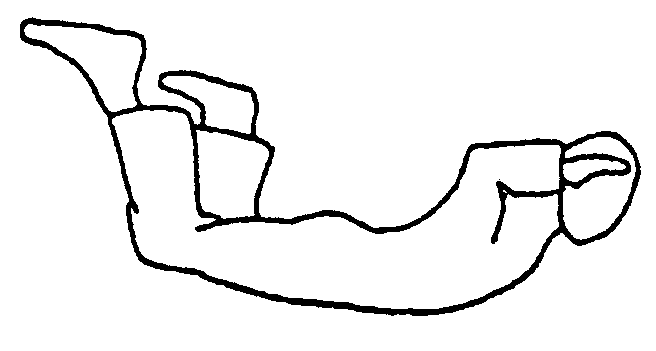
\includegraphics[width=0.7\textwidth]{Asento-perus.png}\captionof{figure}{Vapaapudotuksen perusasento}\end{Figure} 

\section{ Käännös }
\label{perusliikkeet-vapaassa-kaannos}


Käännöksen puoleinen käsi ja hartia painetaan alas. Käännöstä voidaan nopeuttaa vartalon taivutuksella, jalan koukistuksella ja pään kääntämisellä. Käännös tehdään siis seuraavasti: 

\begin{enumerate}[label=\bfseries \arabic*)]
\item  Otetaan kiintopiste 45° edestä maasta, esimerkiksi rakennus. 
\item  Hartialinja painetaan alas halutun käännöksen suuntaan. 
\item  Otetaan perusasento ennen kiintopistettä. 
\item  Vähän ennen kiintopistettä tehdään pieni vastaliike, jotta käännös pysähtyy täsmällisesti. 
\end{enumerate}

\begin{Figure}\centering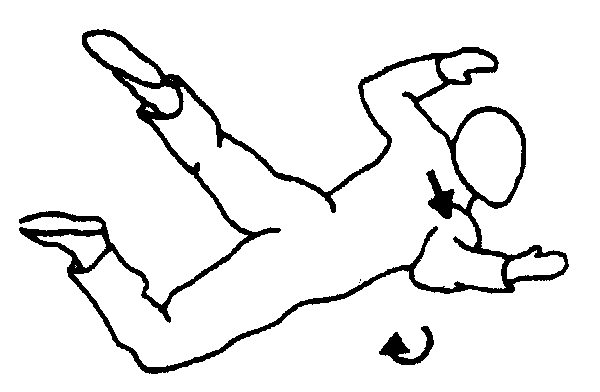
\includegraphics[width=0.7\textwidth]{Asento-kaannos.png}\captionof{figure}{Kääntyminen}\end{Figure} 

\section{ Selkälento }
\label{perusliikkeet-vapaassa-selkalento}


Selkälennon aikana rintahihnassa oleva korkeusmittari ei näytä välttämättä oikein ja vapaapudotusnopeus kasvaa. Jos asennon hallinta menetetään oltaessa selällään (lattakierre), käännetään asento vatsalleen ja otetaan perusasento taivuttamalla. Mikäli asentoa ei saada hallintaan, avataan varjo. Selkälennossa apuvarjo voi irrota löysästä taskustaan tai löysä luuppi voi aiheuttaa varjon ennenaikaisen avautumisen. Selkälento tehdään seuraavasti: 

\begin{enumerate}[label=\bfseries \arabic*)]
\item  Käännetään asento kyljelleen käyttämällä kättä vartalon edessä. 
\item  Taivutetaan samalla asento väärin päin, istuma-asentoon. 
\item  Lennetään muutama sekunti selällään (huomioidaan korkeus). 
\item  Taivutetaan ja käännetään asento käyttämällä kättä vartalossa, jolloin palataan perusasentoon kyljen kautta. 
\end{enumerate}

Palautusta voidaan auttaa ottamalla ensin delta-asento ja vasta kääntymisen jälkeen perusasento. 

\section{ Takavoltti }
\label{perusliikkeet-vapaassa-takavoltti}


Kädet pidetään perusasennossa suorina, hieman sivuille käännettyinä. Jalat laitetaan yhteen ja koukkuun vartalon alle. Painetaan käsillä alaspäin ilmavirtaa vasten. Pysäytys tapahtuu palauttamalla perusasento. Jalkojen nopea ja yhtaikainen tuonti vartalon alle takaa voltin onnistumisen. Käsillä autetaan ympäri menoa ja estetään asennon kallistuminen sivulle. 


Takavoltti tehdään seuraavasti: 

\begin{enumerate}[label=\bfseries \arabic*)]
\item  Vedetään jalat nopeasti yhteen koukkuun. 
\item  Painetaan käsillä alaspäin ilmavirtaa vasten. 
\item  Pään ollessa alaspäin palautetaan perusasento. 
\end{enumerate}

\begin{Figure}\centering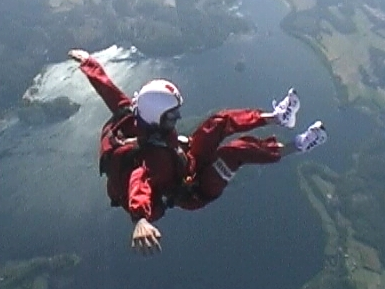
\includegraphics[width=0.9\textwidth]{Selkastabiili.png}\captionof{figure}{Selkälento}\end{Figure} 


\begin{figure*}[]\centering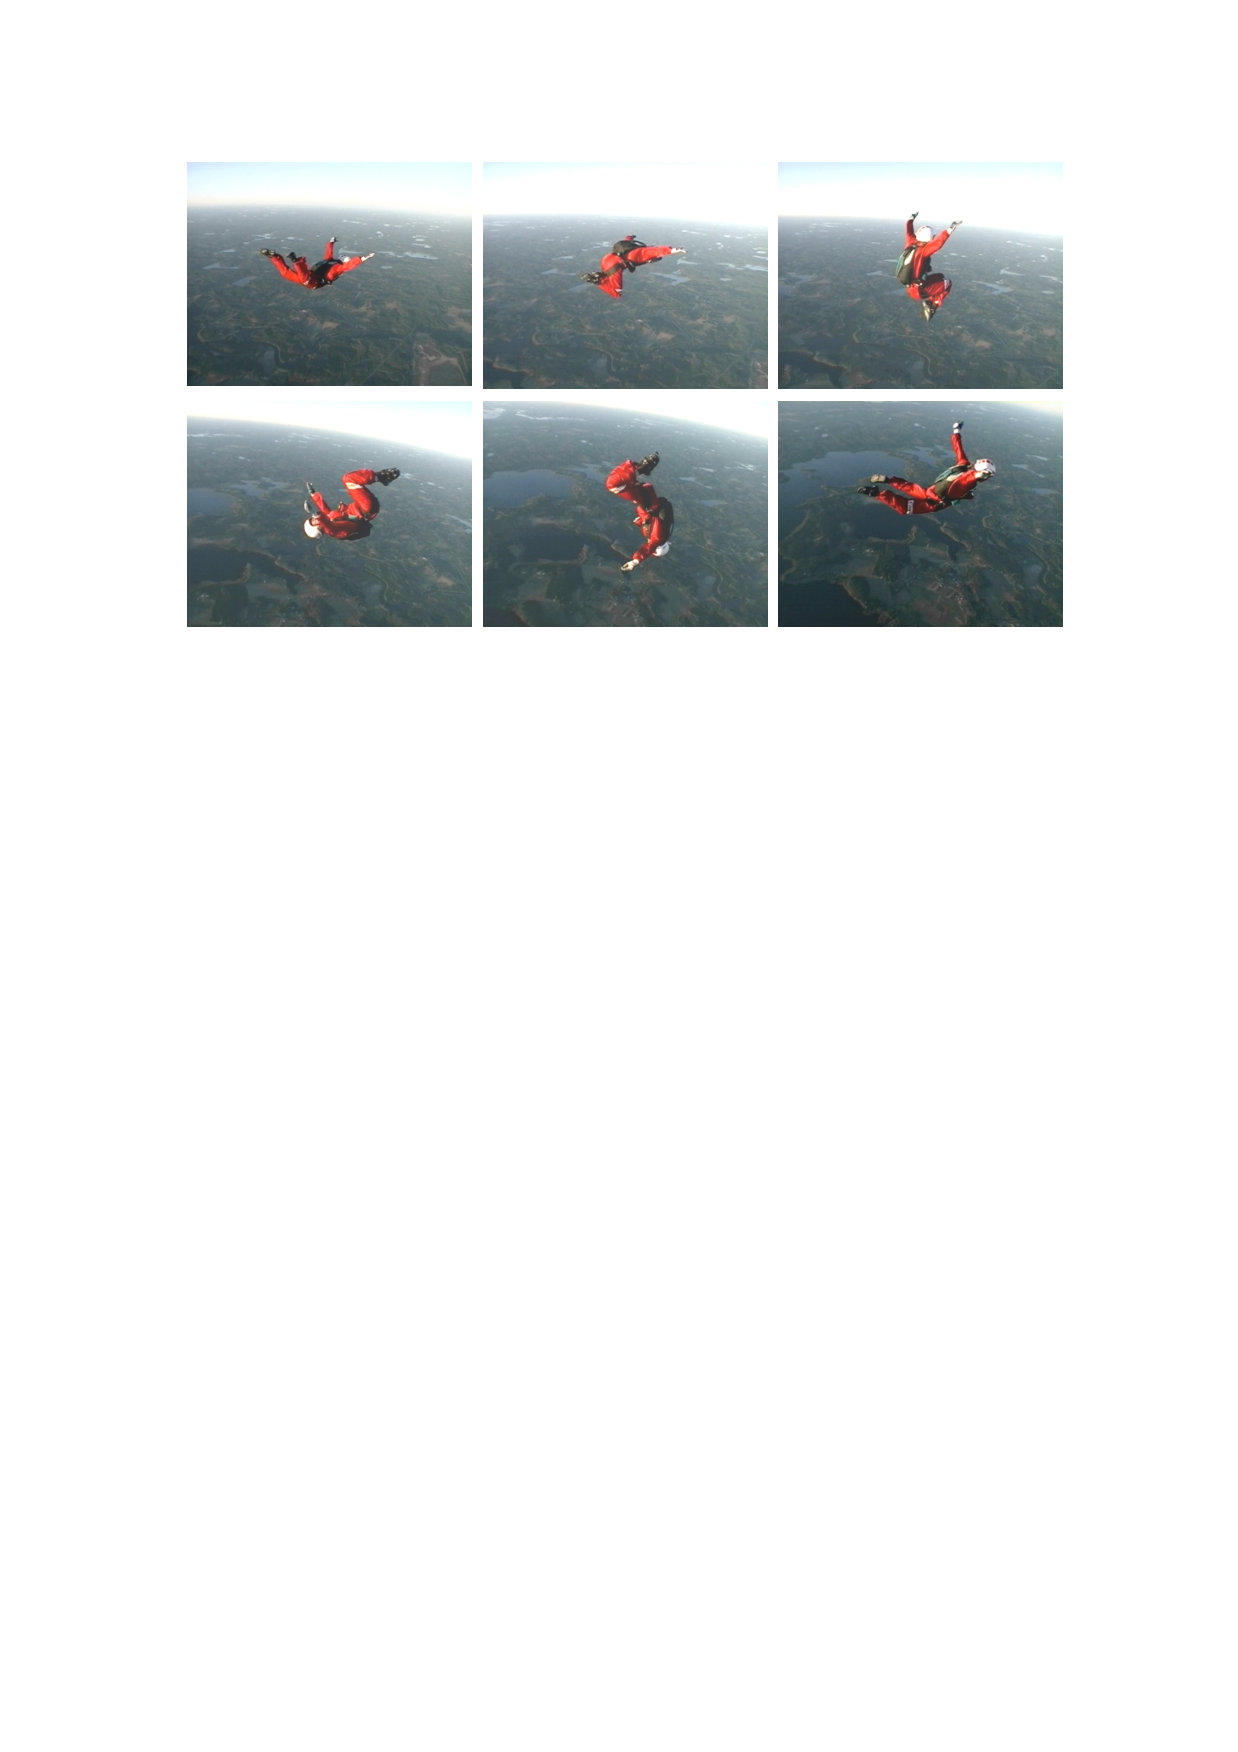
\includegraphics[width=0.95\textwidth]{Takavoltti.pdf}\caption{Takavoltin suoritus}\end{figure*} 

\section{ Tynnyri }
\label{perusliikkeet-vapaassa-tynnyri}


Tynnyri on freeasentojen perusliike, sillä isommilla freekuvilla purun jälkeen liu’uttaessa voidaan tekemällä liu’usta tynnyri tarkastaa vapaa ilmatila ennen avausta. Tynnyrissä on tarkoitus kääntyä vatsaltaan kyljen kautta selälleen ja siitä edelleen täysi kierros takaisin mahalleen. Tynnyri tehdään perusasennosta viemällä toinen käsi vartalon lähelle tai alle ja samalla kääntämällä vartaloa samaan suuntaan vaaka-akselin ympäri. Asennon käännyttyä selälleen jatketaan liikettä kääntymällä toisen kyljen kautta ympäri takaisin perusasentoon. 

\section{ Liuku }
\label{perusliikkeet-vapaassa-liuku}


Liu’un tavoitteena on liikkua vaakatasossa mahdollisimman kauaksi muihin hyppääjiin nähden samalla, kun pudotaan alaspäin. Liuku ei ole siis syöksyä tai tikkaamista. FS-liukuun kuuluvat myös purkumerkki, 180° käännös, liuku vapaaseen suuntaan, liu’un jälkeinen ilmatilan tarkastus sekä avausmerkki ja harjoitusveto. Putoamisnopeus voi kasvaa liu’un aikana. Korkeuden tarkkailu on tärkeää, sillä liu’un pysäytys vaatii myös aikansa. Varjon avaamista suoraan liu’usta ei suositella. Hyvä liuku on ensiarvoisen tärkeä taito laskuvarjohyppääjällä, sillä ainoastaan hyvällä liu’ulla pystyy varmistamaan riittävän välimatkan muihin hyppääjiin purun jälkeen!  Liuku tehdään seuraavasti: 

\begin{enumerate}[label=\bfseries \arabic*)]
\item  Otetaan kiintopiste edestä, maasta. 
\item  Oikaistaan jalat. 
\item  Viedään kädet sivuille taakse, lähelle vartaloa. 
\item  Painetaan olkapäät alas eteen. Hyppääjä on delta-liu’ussa. 
\item  Ohjataan liukusuuntaa kämmenillä. 
\item  Tarkkaillaan korkeutta, muita hyppääjiä sekä liu’utaan kohti kiintopistettä. 
\item  Palautetaan perusasento rauhallisesti ottamalla 
\item  Ensin taivutus = delta-asento 
\item  Palautetaan kädet ja jalat perusasentoon. 
\end{enumerate}

\begin{Figure}\centering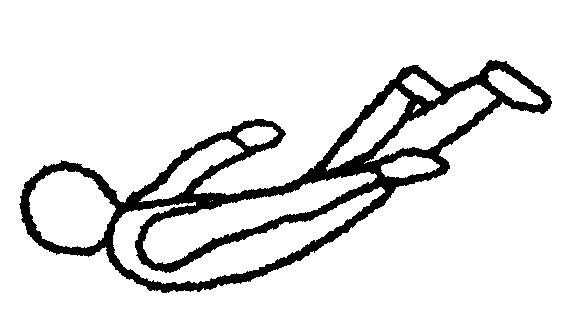
\includegraphics[width=0.7\textwidth]{Asento-deltaliuku.png}\captionof{figure}{Delta-asento}\end{Figure} 


\begin{Figure}\centering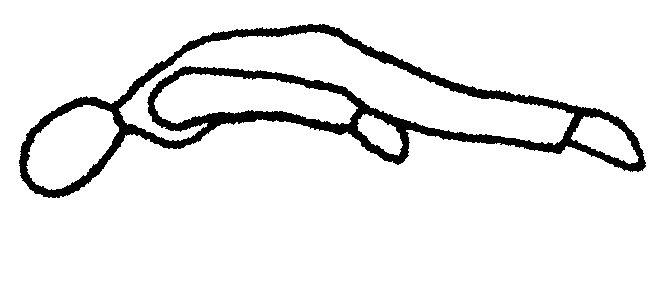
\includegraphics[width=0.7\textwidth]{Asento-liuku.png}\captionof{figure}{Liukuasento}\end{Figure} 


\end{multicols}\pagebreak\begin{multicols}{2} 

\section{ Vaaratilanteet }
\label{perusliikkeet-vapaassa-vaaratilanteet}

\begin{enumerate}[label=\bfseries \arabic*)]
\item  Jäykkyys aiheuttaa asennon heilumista (puun lehden tippumisilmiö). Rentouta asento. 
\item  Epäsymmetrisyys aiheuttaa lattakierrettä. Tee vastaliike. Jos pyöriminen ei pysähdy, avaa varjo heti. 
\end{enumerate}

Lattakierre: 

\begin{itemize}
\item  On holtitonta pyörimistä vaakatasossa 
\item  Aiheutuu epäsymmetrisestä ja jäykästä asennosta tai hallitsemattomasta käännöksestä 
\item  Aiheuttaa asento- ja ajantajun menettämisen 
\item  Pysäytetään rentouttamalla asentoa ja hartialinjan vastaliikkeellä. Jos vastaliike ei auta ja liike ei ole hallinnassa, ota perusasento, taivuta ja avaa varjo heti.  
\end{itemize}

Harjoitukset 

\begin{enumerate}[label=\bfseries \arabic*)]
\item  Katsotaan eri uloshyppyjä Oppilaan Opas -videolta kouluttajan kanssa. 
\item  Harjoitellaan kouluttajan mallien mukaan maassa liike kerrallaan. 
\item  Liikkeiden (delta, liuku ja FS-liuku) harjoittelu laudalla tai vapaapudotusvaljaissa. 
\end{enumerate}
